\chapter{Renderização interativa de dODFs}
\label{chap::renderizacao_interativa_de_perfis_de_difusao}

%\todo[inline]{Falta contextualizar nos objetivos que você listou na seção 1.3. Não é melhor focar em renderização de perfis de difusão que é um dos problemas relacionados diretamente com a interatividade?}

A forma mais comum de visualizar dados  relacionados a ODFs é através de glifos provenientes da superfície definida pela plotagem polar esférica $R(\mathbf{\hat{u}})$. Esta classe de superfície permite a inferência e inspeção de ODFs de difusão e a distribuição de fibras subjacentes. Adicionalmente, permite a avaliação visual das ODFs obtidas a partir de um método de alta ordem para DWI em diferentes esquemas de aquisições. Estes glifos dão uma visualização clara do comportamento local de difusão e são amplamente utilizados para provas de conceito em trabalhos na área HARDI e essenciais para visualização dos resultados gerados pelos métodos de alta ordem.

Entre os trabalhos que utilizam os glifos, temos \citeonline{TuchQBall2004},  \citeonline{yeh2010} e  \citeonline{daducci2014}.  \citeonline{descoteaux2007}. \citeonline{TuchQBall2004},  \citeonline{yeh2010} os utilizam como ferramenta de visualização para os métodos de imageamento propostos em seus respectivos trabalhos. \citeonline{daducci2014} os utiliza para ilustrar e comparar ODFs reconstruídas por diferentes métodos.
%E \citeonline{descoteaux2007} aplicam os glifos  para ilustrar \todo{É isso mesmo?}\textcolor{red}{diferentes formas de visualizar os dados relacionados a dODFs} \sout{transformações entre ODFs}.
Neste trabalho, propomos visualizar as dODFs através dos seus dados min-max normalizados correspondentes. A relação de normalização é detalhada na seção \ref{sec::glifos_odf}.

Além de proporcionar melhor entendimento dos dados adquiridos pelas técnicas de alta ordem, conjeturamos com base nos achados de \citeonline{voltoline2021}, que a visualização das dODFs através de glifos posicionados em seus respectivos \textit{voxels} sobrepostos a um volume de ressonância magnética ponderada em T1 pode melhorar o processo de escolha de sementes para tractografia.

Neste capítulo, apresentamos o algoritmo de renderização interativa de ODFs através de glifos, integrados ao ambiente de visualização multimodal para visualização DWI e MRI anatômico ponderado por T1 co-registrados. Devido à grande quantidade de dados que definem as ODFs, mostramos estratégias para lidar com o potencial alto tráfego de dados CPU-GPU e minimizamos o uso da memória da GPU para renderização dos glifos.

Para isto, propomos uma novo algoritmo de renderização de glifos ODF baseado em triângulos, no qual utilizamos a instanciação de GPU e tiramos vantagem da simetria desta classe de funções para lidar com o gargalo no tráfego de dados CPU-GPU e a limitação da memória de vídeo. Adicionalmente, elaboramos um algoritmo de tesselação recursiva de icosaedro para geração de malhas esféricas de ordem $2^k$  que nos permite  obter um espaço de amostras de orientações \textit{quasi}-igualmente espaçadas na esfera e relacionar a sua área de projeção na tela e resolução, proporcionando um aumento no desempenho temporal sem afetar a qualidade de informação codificada na malha.

\todo[inline]{A revisar \textcolor{green}{OK!}}

O capítulo está organizado em seis seções. Na seção \ref{sec::trabalhos_relacionados}, apresentamos os trabalhos relacionados; na seção \ref{sec::superquadricas}, apresentamos brevemente a \textit{pipeline} de renderização multimodal para visualização de DWIs co-registrados com MRI anatômico ponderado em T1 e glifos ODF e um fluxograma representativo; na Seção \ref{sec::renderizacao_de_glifos_ODF}, apresentamos a o mapeamento dos glifos em uma forma geométrica; na Seção \ref{sec::inicialização_do_algoritmo}, apresentamos os procedimentos de inicialização do algoritmo; na Seção \ref{sec::trafego_cpu_gpu}, apresentamos o papel da CPU no algoritmo de renderização e o leiaute de memória dos dados que são enviados à GPU a cada requisição de desenho; e na Seção \ref{sec::processamento_GPU}, mostramos as tarefas executadas pelos \textit{vertex} e \textit{fragment shaders} na GPU para renderização dos glifos.

%\sout{; na seção \ref{sec::experimentos}, mostramos os experimentos e resultados. Na Subseção \ref{ssec::aspectos_visuais}, mostramos aspectos visuais, em que ilustramos a atuação do modelo que relaciona a ocupância e resolução e mostramos que esses glifos são mais informativos que os superquádricos por permitir o inferimento do cruzamento de fibras e \ref{ssec::performance} atestamos a sua interatividade.}\todo{Cap. 4?}

\section{Trabalhos Relacionados}
\label{sec::trabalhos_relacionados}

Apesar da relevância reconhecida da renderização interativa de dados de ODF em glifos, a comunidade não tem explorado muito esta questão. Para poder atender ao requisito de interatividade, limitaremos-nos a trabalhos que exploram recursos da GPU. Há duas grandes abordagens para renderização de glifos. A primeira é baseada em \textit{ray-casting}, onde a geometria do glifo é representada por uma função ou expressão algébrica \cite{peeters2009, almsick2011}. A outra é baseada na renderização de malhas, com a geometria do glifo aproximada por malhas poligonais \cite{shattuck2008}.

\todo[inline]{Sendo uma dissertação, você deve discutir melhor as técnicas apresentadas em relação à solução dada à lista dos potenciais problemas: volume dos dados, tráfego CPU--GPU, tamanho limitado da memória de vídeo, desempenho na renderização. \textcolor{green}{OK!}}

\citeonline{shattuck2008} tessela uma representação polar de ODF com triângulos, onde a superfície do glifo é gerada através da discretização do seu domínio polar, e sua forma é gerada na CPU através de uma função analítica neste domínio. Os glifos são renderizados por fatia. Com a mudança de malha e parâmetros de visualização, os vértices do glifo são re-computados e reenviados à GPU. A performance relatada é de dez \textit{frames}/s para uma fatia de um volume, no qual cada glifo tem 225 vértices, em uma cena com aproximadamente 2 milhões de triângulos.

Em seu trabalho, \citeonline{shattuck2008} não utilizam programação na GPU. Os vértices dos glifos são gerados na CPU pelo escalonamento de pontos de uma malha esférica pelo valor de ODF aplicados em suas respectivas normais. Os dados que são enviados à GPU consistem nos vértices da superfície em um leiaute que definem polígonos, gerando um tráfego de dados redundante e excessivo.

Em nosso trabalho, a definição da superfície de glifo é a mesma: amostras funções que deformam uma superfície esférica. Porém, em nossa abordagem, armazenamos os dados que definem a superfície do glifo como amostras na CPU e exploramos recursos da GPU e a simetria das funções de dODF para minimizar o tráfego de dados CPU-GPU afim de extrair toda a redundância na estrutura de dados relativa a definição de polígonos através de seus vértices, e, adicionalmente, encontramos estratégias para que o tráfego de dados seja relativos a valores escalares de dODF min-max normalizada ao invés de vértices. Na nossa abordagem, a deformação da superfície esférica é feita de forma paralela na GPU.


\citeonline{peeters2009} apresentaram um esquema de renderização utilizando \textit{ray-casting}. Na CPU, o centro, o raio da esfera delimitadora e o cubo delimitador por glifo são computados. Na GPU, o algoritmo de \textit{ray-casting} é executado por pixel no \textit{fragment shader}. Se o raio lançado para um pixel não intercepta a esfera delimitadora, o fragmento é descartado. Caso contrário, o algoritmo executa uma busca linear com passos discretos para interseção da ODF, modelada a partir de funções base, para com o raio. Eles alcançaram uma melhor performance que o algoritmo apresentado por \citeonline{shattuck2008}. \citeonline{almsick2011} melhorou a busca por interseção utilizando o método numérico \textit{regula falsi} e cilindros delimitadores alinhados com o eixo de visão. Eles atingiram um melhor tempo de performance sem sacrificar a qualidade de renderização, documentando que 9000 glifos puderam ser gerados a 30 FPS. Há um problema crítico na acurácia e eficiência do raio lançado. Quando o raio tende a ser paralelo ao glifo, muitas iterações podem ocorrer em algumas \textit{threads}.

Adicionalmente, na abordagem \textit{ray-casting} em ambos \citeonline{peeters2009} e \citeonline{almsick2011} fazem a consideração que as ODFs sejam definidas como uma soma ponderada de 15 funções base harmônicas esféricas pré-computadas de até quarta ordem. Esta consideração é suficiente para que o usuário possa inferir sobre cruzamentos de fibra, mas é limitante na complexidade da superfície. Os autores não detalham questões relativas à interatividade caso o usuário objetive uma representação gráfica mais complexa utilizando sexta e oitava ordem das harmônicas esféricas, no qual há 28 e 45 funções base \cite{descoteaux2007_QBI}. Neste trabalho, não lidamos com problemáticas desta natureza pois consideramos que as funções são armazenadas via amostras.

Na abordagem \textit{ray-casting}, há uma característica desejável que se refere à independência da qualidade do glifo em função do fator de escala. Em nossa abordagem, escolhemos a malha esférica de forma adaptativa em função da ocupância dos glifos a serem renderizados na tela, para que o processamento realizado por glifo também possa ser adaptativo.

\citeonline{voltoline2021} propuseram um esquema de renderização para glifos superquádricos para tensores de difusão \cite{Kindlmann2004}. Eles exploraram recursos modernos da GPU para atingir este objetivo, que consistem em \textit{transform feedback}, aproximação triangular adaptativa dos glifos e renderização por instanciação indireta. Diferentemente das superquádricas, os dados associados com glifos ODF tem dimensionalidade bem maior, o que inviabiliza seu armazenamento na GPU. Consequentemente, devemos propor estratégias para minimizar o tráfego de dados CPU-GPU para os glifos a serem renderizados, almejando a interatividade.

\section{Renderização multimodal de glifos ODF}
\label{sec::superquadricas}
Nesta seção, descreveremos brevemente o ambiente de renderização multimodal no qual o algoritmo de renderização de glifos ODF é integrado. A Fig. \ref{fig::vmtk_simplified} ilustra o ambiente de visualização.

O algoritmo de renderização é dividido em três estágios: (1) renderização do DWI e do volume anatômico co-registrados; (2) detecção dos \textit{voxels} visíveis e estimativa da cobertura máxima da projeção dos glifos em \textit{pixels}, para estimativa da resolução da malha; (3) estimativa da resolução da malha e renderização de glifos sobrepostos ao seus respectivos \textit{voxels} visíveis na resolução estimada.

\subsection{Ray-casting de volumes múltiplos}

No ambiente, a visualização se dá em torno de ambos volumes DWI $b0$ e MRI anatômico ponderado em T1. Os volumes são co-registrados a partir de uma matriz de co-registro rígido \cite{ting2014}, tendo $b0$ como referência e o MRI T1 como flutuante \cite{voltoline2021}. Os volumes transferidos à GPU e são renderizados via \textit{ray-casting} \cite{kruger2003}, que é uma técnica bem estabelecida para renderização de sinais de MRI.

No \textit{ray-casting}, um raio é lançado por \textit{pixel} sobre o volume de interesse. O processo é iterativo, no qual o raio é amostrado em posições discretas ao longo do caminho no qual o nível de cinza é computado através dos sinais de MRI do volume.

Para cômputo do nível de cinza, há dois atributos gráficos extraídos do volume, que consistem no nível de cinza por \textit{voxel} $C_{src}$ e opacidade $\alpha_{src}$. Ao longo do raio estes atributos são acumulados a partir dos dados da iteração anterior, afim de computar um tom de cinza $C_{dst}$ e opacidade $\alpha_{dst}$, que são inicialmente zerados:

\begin{equation}
    C_{dst} = C_{dst} + (1-\alpha_{dst})C_{src},
\end{equation}
\begin{equation}
    \alpha_{dst} = \alpha_{dst} + (1-\alpha_{dst})\alpha_{src}.
\end{equation}

O processo iterativo é terminado quando acabam as amostras do volume para contribuição na cor do \textit{pixel}, ou quando $\alpha_{dst}$ atinge um limiar de superfície opaca $\alpha_{max}$. O nível de cinza do fragmento e opacidade são definidos como $C_{dst}$ e $\alpha_{dst}$. Fig. \ref{fig::ilustracao_raycasting} ilustra o algoritmo.

\begin{figure}[ht]
\centering
\captionsetup[subfloat]{farskip=0pt,nearskip=0pt}
\centering
   \subfloat[Em vermelho, os raios lançados por pixel. Os pontos indicam o ponto de amostragem do raio no volume, onde o valor do \textit{voxel} $C_{src}$ e $\alpha_{src}$ são extraídos para cômputo de $C_{dst}$ e $\alpha_{dst}$. Os pontos amarelos indicam espaço vazio e os brancos indicam pontos do volume. Por simplicidade, ilustramos para apenas seis \textit{pixels}, enquanto a quantidade real para o plano é dado pelo comprimento da imagem em \ref{fig::raycasting_3d}.
    ]{\makebox[1.7\width]{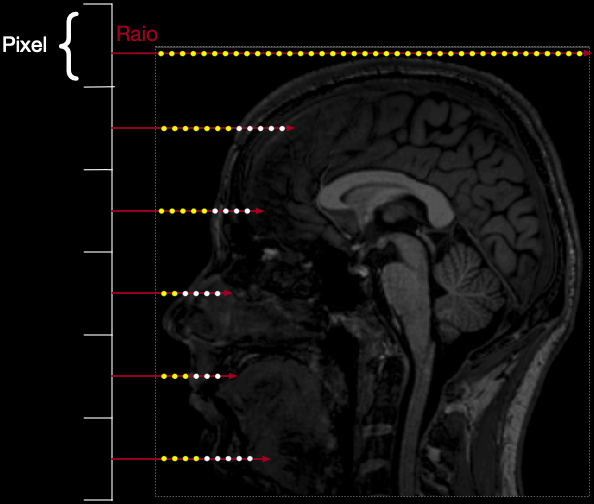
\includegraphics[width=.55\linewidth, angle=0]{figs/Esquema_Glifo/raycasting/raycasting_2d_2.png}
    \label{fig::raycasting_2d}
    }
    }
    \\
    \hspace{1em}
    \subfloat[Volume 3D renderizado via \textit{ray-casting}] {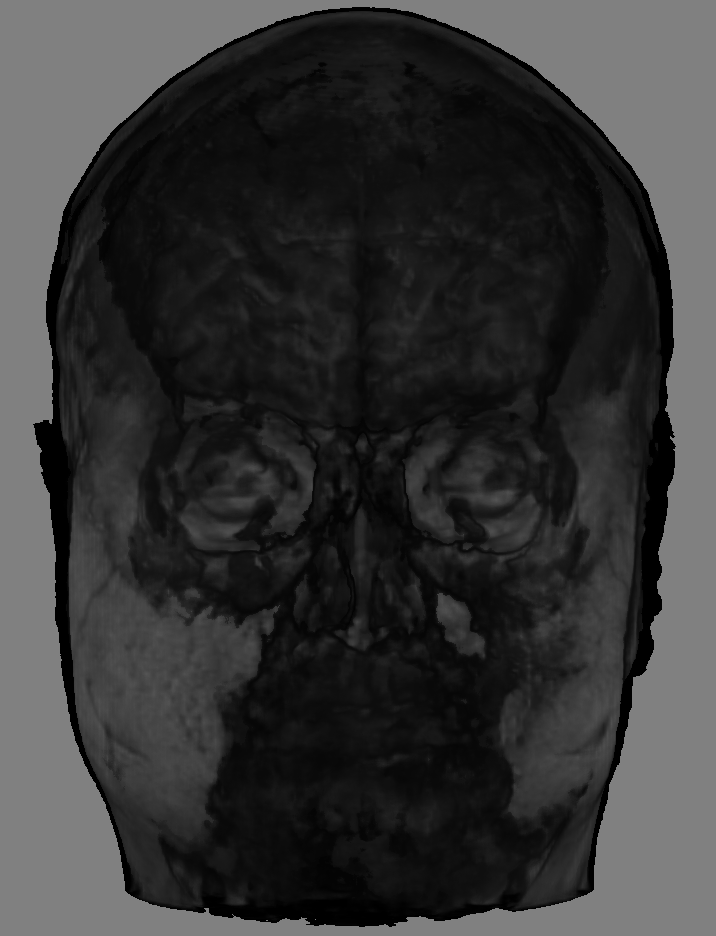
\includegraphics[width=.37\linewidth, angle=0]{figs/Esquema_Glifo/raycasting/raycasting_3d.png}
    \label{fig::raycasting_3d}
    }
     \caption{Ilustração do processo de \textit{ray-casting} de um volume MRI. Fig. \ref{fig::raycasting_2d} ilustra o \textit{ray-casting} para os \textit{pixels} situados em um plano ortogonal à Fig. \ref{fig::raycasting_3d} na coluna central da visualização 3D.}
    \label{fig::ilustracao_raycasting}
\end{figure}

No \textit{ray-casting} de volumes múltiplos, a cor é determinada pela soma ponderada entre dois volumes, que são co-registrados afim de estarem no mesmo espaço tridimensional.

No processo de renderização na GPU dos volumes co-registrados, uma matriz com as dimensões da janela de renderização é definida onde os elementos de coordenada  $(x, y)$ armazenam as coordenadas $(v_x, v_y, v_z)$ do primeiro \textit{voxel} visível atingindo pelo raio no algoritmo de \textit{ray-casting}.

\subsection{Processamento de \textit{voxels} visíveis}

A partir da matriz com as coordenadas dos \textit{voxels} atingidos pelo raio na renderização via \textit{ray-casting} do volume de difusão alocada na GPU, uma lista sem repetição das coordenadas \textit{voxels} visíveis $D = [
\mathbf{d}_1,
\mathbf{d}_2, ..., 
\mathbf{d}_M
]$ e a quantidade de \textit{pixels} ocupada por cada um são computadas.

A partir das da quantidade de \textit{pixels} associadas às coordenadas de cada \textit{voxel}, o valor máximo de \textit{pixels} $max_p$ ocupados por um único \textit{voxel} é extraída. O algoritmo para o cômputo de $max_p$ utilizado neste trabalho pode ser encontrado em \citeonline{voltoline2021}.

\subsection{Renderização de glifos ODF}

Enviamos os conjunto $D = [
\mathbf{d}_1,
\mathbf{d}_2, ..., 
\mathbf{d}_M
]$ de \textit{voxels} visíveis detectados e $max_p$ da GPU para a CPU no qual preparamos os dados pré-computados que sintetizam os glifos a serem renderizados. Enviamos estes dados à GPU para que cada glifo seja sintetizado e renderizado de forma sobreposta ao seu respectivo \textit{voxel}.

O procedimento de pré-computo, a preparação dos dados que sintetizam os glifos, bem como o processamento da GPU para renderização serão apresentados neste capítulo.

 %que cada um ocupa são computados, cujo algoritmo foi proposto por \citeonline{voltoline2021}





%Para manter a compatibilidade do algoritmo com o Mac OSX, cuja versão máxima suportada do OpenGL é 4.1, eles desdobraram o algoritmo para estimação de cobertura máxima de \textit{pixels} para os glifos de um passo, onde a implementação é feita no \textit{compute shader} em um algoritmo de quatro passos, envolvendo \textit{vertex, geometry} e \textit{fragment shaders} baseados em rasterização. Para evitar transferência de dados entre CPU e GPU entre passos, o \textit{transform feedback buffer} foi aplicado. Adicionalmente, eles mostraram a utilização do mecanismo de \textit{additive blending} para obtenção do número máximo de \textit{pixels} ($max_p$), no qual o \textit{voxel} é projetado em um volume \textit{ray-casted}. Baseado em $max_p$, eles estabelecem uma heurística para estimação da resolução da malha.


\todo[inline]{Não seria glifos ODFs? \textcolor{green}{OK!}}

%\citeonline{voltoline2021} propuseram um algoritmo de renderização multimodal de glifos superquádricos sobre o seu respectivo MRI anatômico ponderado em T1. O volume $b0$, seu respectivo MRI T1 e a matriz rígida que co-registra ambos os volumes  são enviadas à GPU.

\todo[inline]{É preciso adequar a figura ao texto. Onde estão os dados 
de instância? Onde está a malha esférica? \textcolor{green}{OK!}}
\begin{figure}[ht]
    \centering
    %\rule{6cm}{3cm}
    \includegraphics[width=.7\linewidth, angle=0]{figs/Esquema_Glifo/fluxograma_glifos_VMTK_5.png}
    \caption{
    Renderização multimodal para glifos ODF. A cor azul representa a saída a ser desenhada, armazenada no \textit{framebuffer} (FB); a cor magenta se refere a dados pré-computados. Os volumes co-registrados são renderizados via \textit{ray-casting} e processamento de \textit{voxels} visíveis estão descritos por \citeonline{voltoline2021}. O estágio de preparação dos dados de ODF e renderização de glifos ODF estão descritos na Seção \ref{sec::renderizacao_de_glifos_ODF}. Os vértices da malha esférica base são armazenados na GPU são replicados por instância. O superconjunto de índices referenciam os vértices afim de formar a malha esférica com diferentes resoluções. As setas preta indicam entrada e saída de dados computados nos módulos apresentados.
    }
    \label{fig::vmtk_simplified}
\end{figure}





%Através de $max_p$, um \textit{tessellation shader} é acionado para gerar o \textit{skeleton} base dos superquádricos, no qual eles utilizam o comando renderização indireta por instâncias para desenhá-los com uma chamada desenho. Provendo a parâmetros particulares a cada \textit{voxel} que definem cada superquádrico, em cada instância o \textit{skeleton} é customizado para gerar o glifo e é posicionado em seu respectivo \textit{voxel} no espaço do volume.


\section{Mapeamento dos glifos ODF em formas geométricas}
%\section{Renderização de Glifos ODF}
\label{sec::renderizacao_de_glifos_ODF}

\todo[inline]{Não ficaria melhor $S$, como no cap. 2? \textcolor{green}{Eu apresento S como um domínio de amostragem da SDF, dODF e min-max dODF, já N é a quantidade de pontos da malha. No nosso caso, S = N/2, já que amostramos no hemisfério}} 
\todo{Nossa proposta? Ou já é uma ideia antiga? Cite uma referência. \textcolor{green}{No material que vejo, essa abordagem malha esférica deformada não há referência. O Peeters chama ela de abordagem tradicional}}

A fim de renderizar os dados numéricos de dODFs min-max normalizadas em GPUs, é necessário mapear estes dados em atributos de modelos geométricos processáveis pelas GPUs. Utilizamos a forma tradicional para geração da superfície do glifo \cite{peeters2009}, cuja superfície é gerada pela deformação de uma malha esférica unitária, cujos os vértices $\Pi = \{
P_1$,
$P_2$, ...,
$P_N
\}$, são escalonados pela dODF min-max normalizada $R(\mathbf{r}, \mathbf{n}_i)$, onde $\mathbf{n}_i$ é unitário e tem direção e sentido de $P_i \in \Pi$. Após a definição da superfície do glifo, o escalonamos para estar contido no domínio de cada \textit{voxel}, e os deslocamos para o centro do seu respectivo \textit{voxel} de coordenadas $\mathbf{r}$ na cena, como mostrado na Fig. \ref{fig::esfera_deformada_cena}.

\begin{figure}[htb]
    \centering
    %\rule{6cm}{3cm}
    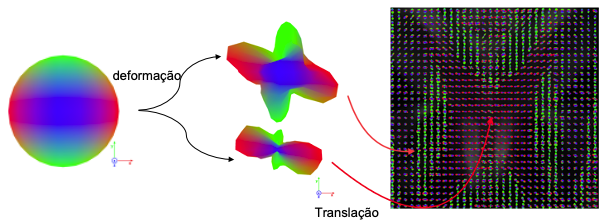
\includegraphics[width=1.0\linewidth, angle=0]{figs/Esquema_Glifo/Renderizacao_multimodal.png}
    \caption{
    Os glifos são gerados a partir da deformação da esfera a esquerda e então escalonados e posicionados na cena.
    }
    \label{fig::esfera_deformada_cena}
\end{figure}

%Em nossa abordagem, a geração da superfície, escalonamento e deslocamento dos glifos ocorre na GPU, a partir de uma malha esférica. %com o deslocamento dos seus $N$ vértices, centrada em $\mathbf{r}$, em função de \textcolor{red}{$\psi_m (\mathbf{r, \mathbf{n}_i}) \mathbf{n}_i$, onde $\mathbf{n}_i$ é o vetor normal à malha esférica no ponto $P_i$ e $\psi (\mathbf{r, \mathbf{n}_i})$ é a função de distribuição de difusão (dODF) min-max normalizada. distribuição de \textit{spin} (SDF) de orientação $\mathbf{n}_i$, seguindo o procedimento apresentado na seção~\ref{sec::glifos_odf}}. \sout{Para uma malha esférica cujo conjunto de vértices é dado por $\{
%P_1,
%P_2, ...,
%P_S
%\}$, o glifo de uma ODF $R(\mathbf{\hat{u}})$ é gerado pelo escalonamento de cada um dos pontos $P_K$ da malha $(1 \leq K \leq S)$ pelo seu respectivo $R(\mathbf{n_K})$, onde $\mathbf{n_K}$ é o vetor unitário com direção e sentido da normal do ponto na esfera em $P_K$.} 

Na CPU, geramos as malhas esféricas base e computamos o conjunto de dODF min-max normalizadas para todos os \textit{voxels} do volume. Como os espaços de memória da CPU e GPU são distintos, esses dados precisam ser transferidos para GPU antes da renderização dos glifos. Nesta seção vamos discutir a nossa proposta para representar os dados de dODF min-max normalizada que leva em consideração o tráfego entre CPU e GPU e a limitação da memória de vídeo.

% A ODF associada a um \textit{voxel} é tipicamente representada por um conjunto de $N$ amostras de difusão $[
% R(\mathbf{\hat{n}}_1), 
% R(\mathbf{\hat{n}}_2), ...,
% R(\mathbf{\hat{n}}_{N-1}),
% R(\mathbf{\hat{n}}_N)
% ]^T$, onde cada $\mathbf{\hat{n}}_i$ é tem a direção e sentido da normal de cada ponto $ P_i$ de uma malha esférica. O glifo é sintetizado pelo deslocamento de cada ponto $P_i$ pelo seu escalar associado $R(\mathbf{\hat{n}}_i)$. Todas as amostras e ODF são computadas, conforme mostrado no Capítulo \ref{chapter::metodos_hardi} e acessíveis pelos seus respectivos ínndices de \textit{voxel}.

%\subsubsection{Simetria}

Tomando vantagem da simetria das funções do sinal de difusão em relação aos eixos coordenados \cite{descoteaux2015}, e da propriedade da malha esférica obtida com o procedimento de subdivisões sucessivas de um icosaedro apresentado na seção \ref{ssec::dominio_esferico} na qual cada vértice presente na malha é acompanhando de sua antípoda, podemos amostrar dODFs usando somente os dados de uma malha semi-esférica.

Propomos categorizar em pontos com subíndice ímpar $\Pi_{impar} = \{P_1$,
$P_3$, ...,
$P_{N-3}$,
$P_{N-1}\}$ nos pontos contidos no hemisfério $\{P(x, y, z) \in \Pi | y > 0 \cup (y = 0 \cap x > 0)\}$, e o restante dos pontos da malha esférica em $\Pi_{par} = \{P_2, P_4, ..., P_{N-2}, P_{N}\}$. Além disso, condicionamos que $P_{2i+2} = -P_{2i+1}$, $(0 \leq K \leq \frac{N-2}{2})$, de forma que os vértices $P_{2i+2}$ e $P_{2i+1}$ sejam vértices antipodais. Assim, para uma malha esférica com $N$ vértices, os dados do conjunto de direções $\mathbf{U}_{3\times \frac{N}{2}} = [
\mathbf{n}_1,
\mathbf{n}_3, ..., 
\mathbf{n}_{N-3},
\mathbf{n}_{N-1}
]$, são suficientes para moldar um glifo. Fig. \ref{fig::direcoes} ilustra a amostragem no conjunto $\mathbf{U}$ a partir dos pontos na semi-esfera definida por $\Pi_{impar}$.

Pelos testes realizados, recomendamos que a ordem de tesselação para amostragem seja a oitava ou, no máximo, a décima sexta, implicando em 321 e 1281 amostras de dODFs min-max normalizadas por \textit{voxel}. Valores acima destes computados para todo DWI pode incorrer no uso de uma quantidade proibitiva de memória. Por exemplo, para tesselação de oitava ordem, em que armazenamos os dados em um ponto flutuante de 4 \textit{bytes}, são necessários 1.284 bytes por \textit{voxel}, que gera aproximadamente 4.480 \textit{Gigabytes} de memória para um volume de dimensões $145 \times 174 \times 145$ do \textit{Human Connectome Project} \cite{essen2012}.

%\subsection{Geometria base}

%\subsubsection{Considerações iniciais}
%\subsubsection{Multiresolução}

%\sout{As ODFs são amostradas a partir dos vetores normais dos pontos de uma malha base esférica $(\Pi, I)$, onde $\Pi = [P_1, P_2, \dots, P_N]$ consiste num conjunto de pontos não repetidos e o conjunto $I$ são os índices que referenciam os pontos de $\Pi$ para formar os triângulos que sintetizam a malha. Estabelecemos duas condições para a estrutura de dados, nas quais tiramos proveito da simetria de dados das ODFs e para que façamos a malha ser adaptativa para parâmetros de visualização. Estas condições tem impacto direto no tráfego de dados CPU-GPU, conforme discutido na Subseção \ref{ssec::atributos}.}

%\sout{A primeira condição, conforme já discutido no capítulo \ref{chapter::metodos_hardi} na forma de armazenamento de dados da ODF tira vantagem da simetria e armazena os pontos em metade de uma esfera. Propomos que os pontos simétricos em relação aos eixos coordenados de $\Pi$ estejam dispostos de forma consecutiva na memória, i. e. $P_{2i+2} = -P_{2i+1}$, $(0 \leq i \leq \frac{N-2}{2})$, o que nos leva a uma estrutura de dados $\Pi = [P_1, -P_1, P_3, -P_3, \dots, P_{N-3}, -P_{N-3}, P_{N-1}, -P_{N-1}]$.}

Em vista do custo da memória, é desejável que a ordem de tesselação seja adaptativa na renderização de glifos, de ordem 0 até 16$^a$ ordem. Propomos que os vértices sejam estruturados numa estrutura linear em $\Pi$. Como os vértices da ordem $2^{k+1}$ contêm os vértices da ordem $2^{k}$, propomos anexar, em bloco, os vértices adicionais da ordem $2^{k+1}$ em relação à ordem $2^k$ ao bloco dos vértices da ordem $2^k$, mantendo a relação de vértices de índices pares e ímpares, ou seja $P_{2i+2} = -P_{2i+1}$. Com isso, garante-se que todos os vértices de uma ordem específica sejam contíguos e que os vértices incrementais de sub-malhas de ordens inferiores estejam organizados em blocos facilmente distinguíveis.

%\sout{A segunda condição objetiva fazer a geometria base do glifo ser adaptativa como uma sub-malha da malha esférica base. Seja $k$ o número de sub-malhas de $(\Pi, I)$, onde cada sub-malha é denotada por $(\Pi_i, I_i)$,  $(0 \leq i < k)$, adicionalmente, o número de pontos das sub-malhas é crescente de acordo com os sub-índices, i.e. se $(0 \leq i < j < k)$, implica $|\Pi_j| > |\Pi_i|$. Sugerimos que cada sub-malha $(\Pi_i, I_i)$ seja simétrica em relação a origem e os primeiros $|\Pi_i|$ elementos na estrutura de dados de $\Pi$ corresponda aos elementos de $\Pi_i$. Note que esta condição também implica que, para $i$, $j$ tais $0 \leq i < j < k$, $\Pi_i$ é subconjunto de $\Pi_j$.}

Propomos definir cada triângulo da malha esférica usando os índices dos vértices na lista de pontos $\Pi$. Isso facilita o reuso das coordenadas dos pontos na definição de vários triângulos, evitando duplicação de dados na memória. %Adicionalmente, propomos que a alternância de malhas de malhas ocorra em tempo de execução a partir da escolha do conjunto de índices que referenciam os dados de $\Pi$ afim de aproximar esfera pelas tesselações de ordem $0$, $2$, $4$, e assim por diante.

\subsection{Um Algoritmo de Tesselação}
%\subsubsection{Formulação da geometria e estruturação de dados}
\label{sssec::formulação_da_geometria_e_estruturação_de_dados}

Conforme mencionado no capítulo \ref{chapter::metodos_hardi}, escolhemos o conjunto de malhas derivada da $2^k$-ésima ordem de tesselação do icosaedro. O algoritmo para obtermos a tesselação de $2^k$-ésima ordem é um processo iterativo, repetido em $k$ vezes, que se inicia com o icosaedro. Cada triângulo da malha é subdividido em quatro em cada iteração, onde os novos novos vértices adicionados são computados pela projeção da mediana dos pares de pontos conectados por uma aresta na esfera.

Assim, o conjunto de vértices $\Pi$ da $2^k$-ésima ordem contém todos os vértices das iterações anteriores. Adicionalmente, para cada vértice há um vértice simétrico em relação aos eixos correspondente. O processo de subdivisão de um triângulo está ilustrado na Fig. \ref{fig::icosaedro_faces_2} e um algoritmo para se obter esta categoria de malha pode ser encontrado em \citeonline{luna2012}. Porém, o algoritmo de tesselação do icosaedro apresentado por \citeonline{luna2012} insere muitos vértices repetidos, visto que os pontos medianos computados a cada segmento ocorrem mais de uma vez, dado que dividem duas faces.

%\textcolor{red}{e usa comparações em ponto flutuante para tomadas de decisão, muito sensíveis aos erros de arredondamento.}

Propomos implementar um algoritmo de tesselação em que os novos vértices de subdivisão sejam inseridos apenas uma única vez e que as tomadas de decisão sejam baseadas em operações com números inteiros. Para isso, uma lista de arestas é usada. Para cada triângulo da malha esférica, determina-se os pontos médios das suas três arestas para construir os 4 novos triângulos. A lista de arestas é acessada. Se uma aresta já se encontra na lista de arestas, acessa-se o índice do ponto médio da aresta e remova a aresta da lista de arestas. Do contrário, computa-se o ponto médio da aresta, adiciona-se na lista de pontos este ponto médio e o seu ponto simétrico em relação ao centro, e insere-se na lista de arestas a aresta com os índices dos seus vértices e o índice do novo ponto médio.

A cada processo de subdivisão, guardamos cada conjunto de índices $I_0$, $I_1$, $I_2$, ..., $I_k$ que referenciam $\Pi$ e triangulam a malha esférica afim de aproximar a esfera para a subdivisão de ordem $2^0$, $2^1$, $2^2$ ...,$2^k$, respectivamente. Fig. \ref{fig::icosphere} ilustra malhas esféricas obtida com o algoritmo proposto.

\section{Inicialização do algoritmo}
\label{sec::inicialização_do_algoritmo}

Após a tesselação do icosaedro e antes da renderização dos glifos, definimos o domínio de amostragem das dODFs min-max normalizadas $\mathbf{U} = [
\mathbf{n}_1$,
$\mathbf{n}_3$, ...
$\mathbf{n}_{N-3}$,
$\mathbf{n}_{N-1}]$, onde $\mathbf{n}_i$ é o vetor unitário com direção e sentido de $P_i \in \Pi_{impar}$
e as computamos para todos os \textit{voxels} da aquisição DWI, como mostrado na Seção \ref{sec::gqi} e \ref{sec::vis_dODFs}.

Pela alta dimensionalidade das dODFs min-max normalizadas $\boldsymbol{R}(\mathbf{r}, \mathbf{n})$, as mantemos na CPU, e em tempo de execução da renderização, as enviamos sob demanda para GPU para definição das superfícies dos glifos, o que potencialmente gera um elevado tráfego de dados no processo, que afeta a performance e interatividade da renderização, nos quais discutimos na Seção \ref{sec::trafego_cpu_gpu}.

Para ajustar o tamanho dos glifos ao tamanho dos seus respectivos \textit{voxels}, redimensionamos os glifos com base nos espaçamentos entre \textit{voxels} da aquisição \cite{voltoline2021} com base em um fator de escala dado por $mS/2$, onde
\begin{equation}
    mS = min(spacing_x, spacing_y, spacing_z),
\end{equation}
sendo  $spacing_x$, $spacing_y$, $spacing_z$ é o espaço entre duas amostras adjacentes nos eixos x, y e z, respectivamente. Enviamos $mS/2$ à GPU como uma variável uniforme.



%potencialmente pode afetar a performance do algoritmo de renderização devido à elevada quantidade de dados.


%\begin{figure}[htb]
%    \centering
%    %\rule{6cm}{3cm}
%    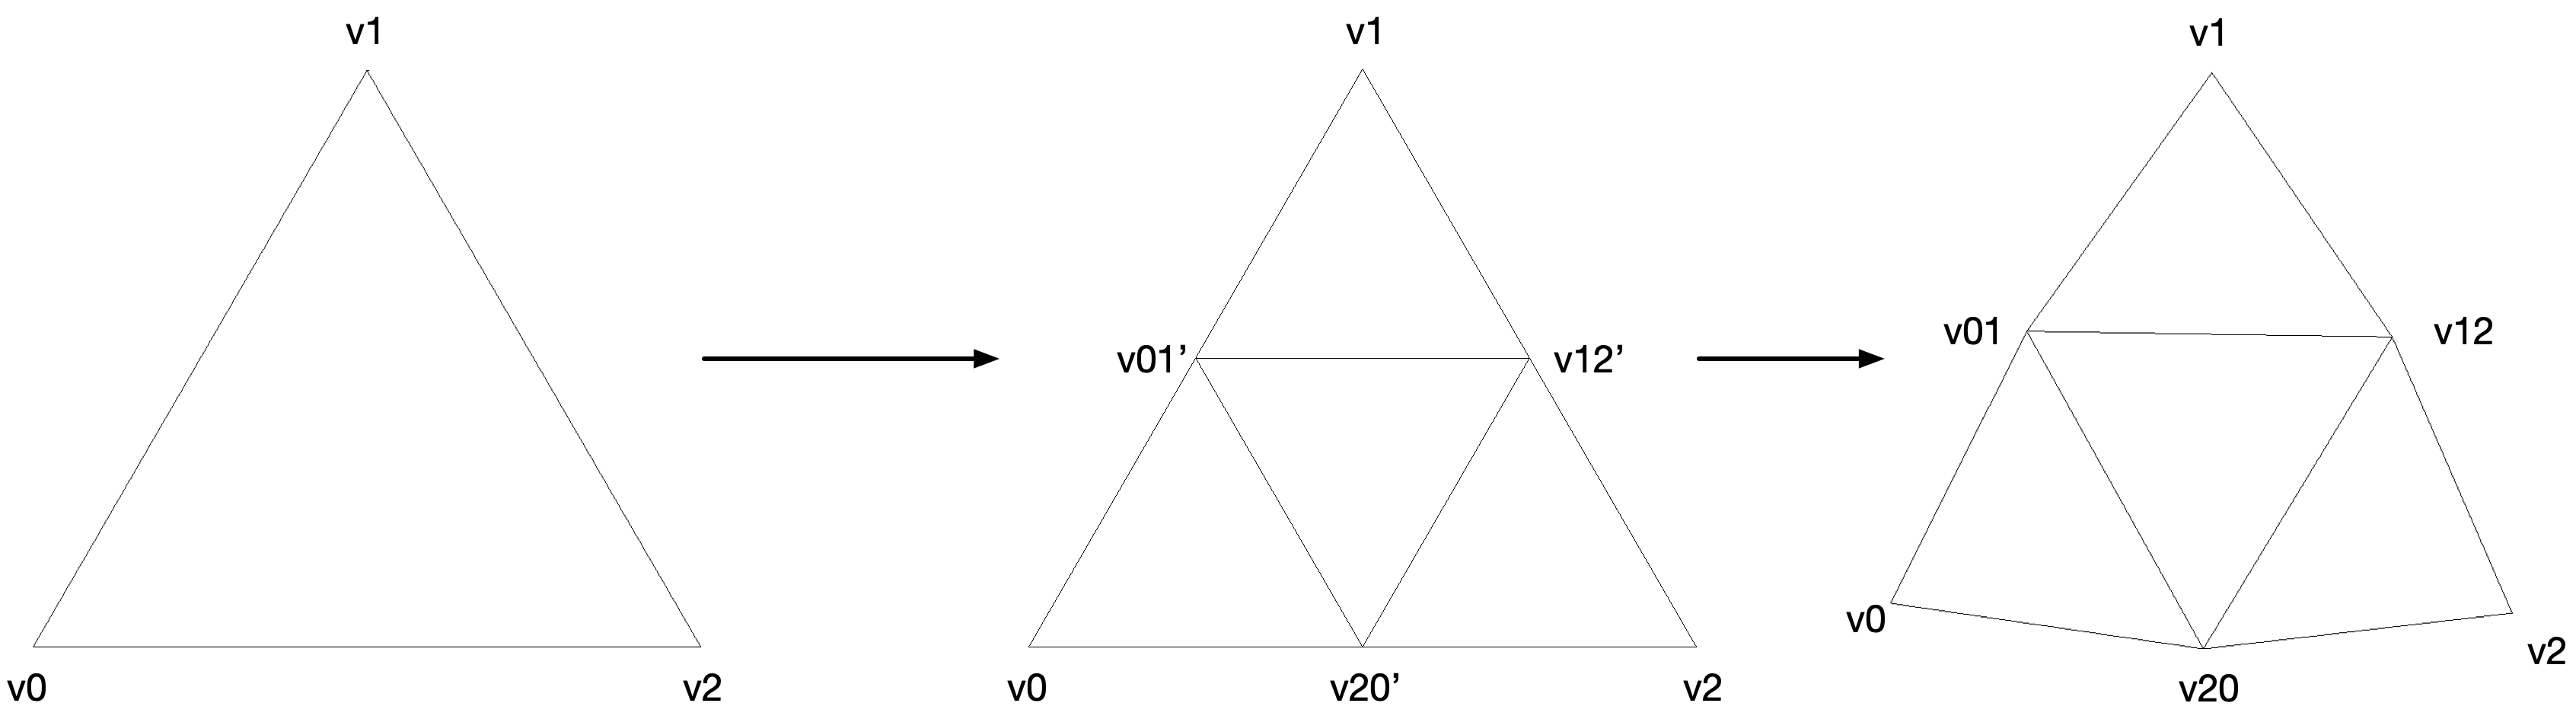
\includegraphics[width=1.0\linewidth, angle=0]{figs/Esquema_Glifo/ico_subdivision.png}
%    \caption{
%    Subdivisão de um triângulo para formar quatro na formação da malha esférica a partir da tesselação de $2^k$-ésima ordem a partir da partir da $2^{k-1}$-ésima. O triangulo formado pelos vértices $v0$, $v1$ e $v2$ é subdividido em quatro, onde as medianas  $v01'$, $v12'$ e $v20'$ são computadas e suas respectivas projeções na esfera $v01$, $v12$ e $v20$ são adicionados ao conjunto de vértices.
%    }
%    \label{fig::triangle_icosahedron}
%\end{figure}

%\sout{Assim como mencionado no capítulo \ref{chapter::metodos_hardi}, por questões de memória, recomendamos k = 3, ou no máximo 4. Assim, formulamos a estrutura de dados que satisfaz as duas condições que estabelecemos a princípio, e é tal que os primeiros 12 elementos correspondem aos vértices do icosaedro, os 42 primeiros elementos correspondem aos vértices da $2^a$ ordem de tesselação, os 162 primeiros elementos correspondem a $4^a$ ordem de tesselação, os primeiros 642 elementos correspondam a $8^{a}$ ordem de tesselação, e, adicionalmente, os pontos simétricos são agrupados em sequencia na memória.}

%\sout{A estrutura de dados $\Pi$, e $I$, além dos índices que triangulam todas as sub-malhas, contidos ao superconjunto $\mathbf{I}$ no Algoritmo \ref{alg::setIcosahedroBase}, são enviados à GPU uma vez. Uma vez que os dados estão na GPU, e visando eficiência no processamento, sem comprometer a qualidade visual, escolhemos adaptativamente a geometria base entre estas malhas por um procedimento heurístico computado em tempo de execução baseado em $max_p$.}

\section{Tráfego CPU-GPU}
\label{sec::trafego_cpu_gpu}

Os espaços de memória da CPU e GPU são distintos. Para renderizar glifos ODF sobre um domínio de orientações especificadas por uma malha esférica da ordem 2$^k$, é necessário transferir a malha esférica e as dODFs min-max normalizadas das amostras visíveis computadas na CPU para GPU. Embora a qualidade dos glifos renderizados aumenta com a resolução da malha esférica, mostramos na seção \ref{sec::renderizacao_de_glifos_ODF} que o volume de dados relativos a dODFs min-max normalizadas cresce exponencialmente com a ordem de tesselação da malha, incorrendo em gargalos na transferência de dados entre CPU--GPU. Abordamos as seguintes soluções para enfrentar o problema de tráfego de dados, devido à alta dimensionalidade das dODFs:

\begin{enumerate}
    \item a renderização dos glifos ocorre sob demanda a partir de um conjunto de $M$ \textit{voxels} visíveis detectados, representados pelo conjunto de coordenadas $D_{3 \times M} = [
\mathbf{d}_1,
\mathbf{d}_2, ..., 
\mathbf{d}_M
]$;
\item escolhemos uma malha esférica a ser deformada dentre as tesselações de ordem $2^1$, $2^2$, ... $2^k$ do icosaedro\footnote{Em nossos testes, o conjunto de índices $I_0$ que sintetiza o icosaedro, que tem 12 vértices, não sintetiza os glifos ODF de forma razoável.} em função da área de cobertura das projeções das malhas esféricas sobre o plano de imagem e apenas os dados que deformam a malha escolhida são enviados para GPU;
\item utilizamos o recurso de instanciação da GPU, para que a superfície do glifo seja gerada a partir de uma malha instanciada já carregada na GPU; e
\item tomamos vantagem da simetria da dODF min-max normalizada, para que o tráfego de dados relativo à geração das superfícies seja referente à metade de uma esfera para definição da superfície.
\end{enumerate}





%\sout{Devido às restrições quanto ao tráfego de dados entre CPU e GPU e à memória em GPUs, três estratégias foram propostas para reduzir o volume de dados: configuração simétrica dos vértices da malha, renderização indexada e instanciação.}



%não só numa demanda proibitiva da memória da GPU e num tempo de processamento excessivo como também 

%\sout{Este procedimento causa uma penalidade em performance devido ao tráfego de dados CPU-GPU devido as mudanças frequentes nas imagens renderizadas em função da interação com o usuário. Assim, nesta seção, apresentamos estratégias para enfrentar esta transferência afim de obter a renderização de forma interativa.
%}

Para que possamos utilizar o recurso de instanciação da GPU, transferimos o conjunto de vértices $\Pi = [
  P_1$,
$-P_1$,
$ P_3$,
$-P_3$,...,
$ P_{N-1}$,
$-P_{N-1}]$ para GPU como um atributo a ser replicado a cada instância, em adição ao superconjunto de índices $\{I_1$, $I_2$, ..., $I_k\}$ antes da inicialização da renderização.

Com os dados das dODF min-max computados e armazenados na CPU e $\Pi$, e o super conjunto de índices $\{I_1$, $I_2$, ..., $I_k\}$ armazenados na GPU, na Seção \ref{malha_esferica} mostramos o procedimento da escolha malha esférica instanciada e na Seção \ref{ssec::atributos}, mostramos o tráfego de dados CPU-GPU que customizam os glifos em uma requisição de desenho a partir do conjunto de \textit{voxels} visíveis $D = [
\mathbf{d}_1,
\mathbf{d}_2, ..., 
\mathbf{d}_M
]$.


%Outra estratégia que adotamos é enviar para GPU somente dados de amostras visíveis com uma resolução adaptativa 

\subsection{Malha Esférica}
\label{malha_esferica}
%\subsection{Escolha automática da geometria base}
%\label{sssec::escolha_automatica_da_geometria_base}
\todo[inline]{Rever o texto destacado abaixo. Caso a estimativa seja baseada me $max_p$, sugir que desse uma ideia como max\_p é estimado ... \textcolor{green}{OK! Feito na seção de overview de ray-cast -> detecção -> renderização} }

\textcolor{magenta}{
A escolha da malha esférica para formação dos glifo é baseada no \textit{trade-off} empírico de \citeonline{voltoline2021}, que indica a quantidade mínima de triângulos $\tau$ para um dado $max_p$ que não sacrifica a qualidade de imagem dos glifos
}
\begin{equation}
\label{eq::trade_off}
    \frac{max_p}{\tau} \geq \sqrt{\frac{max_p}{64}}.
\end{equation}
Reajustamos a inequação para estabelecer uma quantidade mínima de triângulos em função de $max_p$
\begin{equation}
\label{eq::trade_off_2}
    \tau \geq 8\sqrt{max_p}
    .
\end{equation}
 Para explicitarmos a ordem de tesselação na derivação da expressão que escolhe a malha esférica, derivamos a quantidade de triângulos da Eq. \ref{eq::icosphere_triangulos} para $2^t$-ésima ordem de tesselação do icosaedro
\begin{equation}
\label{eq::triangulo_icosaordem}
    \tau = 20\times 4^t
\end{equation}
A partir do \textit{trade-off}, derivamos uma expressão que visa encontrar uma relação entre $max_p$ e a ordem de tesselação do icosaedro a ser utilizada para geração do glifo. Para isso, a partir da desigualdade da Eq. \ref{eq::trade_off}, derivamos uma expressão que relaciona a quantidade de triângulos e $max_p$, onde o icosaedro é mapeado em $max_p = 0$:
%\begin{equation}
%\label{eq::maxp_triangulo}
%    \frac{max_p}{\tau - \tau_{min}} = \sqrt{\frac{max_p}{64}},
%\end{equation}
\begin{equation}
\label{eq::maxp_triangulo}
    \tau - \tau_{min} = 8\sqrt{max_p}
\end{equation}
onde $\tau_{min}$ é a quantidade de triângulos mínimas dentre as malhas a serem escolhidas, que é o do icosaedro e é igual a 20. Aplicando Eq. \ref{eq::triangulo_icosaordem} em  \ref{eq::maxp_triangulo}:
% \begin{equation}
% \label{eq::maxp_order_1}
%     \frac{max_p}{20 \cdot 4^t - 20} = \sqrt{\frac{max_p}{64}}.
% \end{equation}
\begin{equation}
\label{eq::maxp_order_1}
    20 \cdot 4^t - 20 = 8\sqrt{max_p}
    .
\end{equation}
Reestruturando a Eq. \ref{eq::maxp_order_1} para que possamos obter a ordem de tesselação $2^t$ em função de $max_p$, obtemos:
\begin{equation}
\label{eq::icosa_order}
     t = \lceil \frac{1}{2}\log_2{(\frac{2}{5}\sqrt{max_p} + 1)} \rceil,
\end{equation}
onde o arredondamento de $t$ para o próximo valor inteiro garante que o \textit{trade-off} da Eq. \ref{eq::trade_off} seja cumprido. Adicionalmente, $t$ é delimitado pela ordem de tesselação utilizada para amostragem dos dados.

A escolha da malha esférica da tesselação do icosaedro de ordem $2^t$ ocorre na ativação do \textit{index buffer} $I_t$, já carregado na GPU. Há um procedimento adicional que consiste em setar a quantidade de dados de dODF min-max normalizada por glifo enviado à GPU como uma função de sua quantidade de vértices, o que será discutido mais a frente, na Seção \ref{ssec::atributos}.
%%%%%%%%%%%%%%%%%%%%%%%%%%%%

%$\tau \geq 8\sqrt{max_p}$, ($max_p > 0$). 
%Este \textit{trade-off} estabelece a quantidade mínima de triângulos a ser utilizada na malha que não sacrifica a qualidade de imagem dos glifos. Derivamos uma expressão para a escolha da sub-malha da malha esférica base a partir do caso de igualdade do \textit{trade-off}, no qual substituímos a quantidade de triângulos como uma função da ordem de tesselação do icosaedro e mapeamos o icosaedro para o caso $max_p = 0$. A expressão base está na Eq. \ref{eq::icosa_order_base}:


%\begin{equation}
%\label{eq::icosa_order_base}
%     20\times 4^k - 20\times 4^0 = 8\sqrt{max_p}
%\end{equation}


%\textcolor{magenta}{Derivamos $t$ ($t \leq k$) na Eq. \ref{eq::icosa_order} como a ordem de tesselação do icosaedro escolhida. Como $t$ é inteiro positivo, para satisfazer o \textit{trade-off} de \citeonline{voltoline2021}, arrendondamos o valor para cima.}

%The vertices and amount of triangles and the expression for the vertices and triangles number for each $2^k$ tessellation are in Table \ref{tab::icosahedron_set}. In practice, we recommend $k$ to be equal to 3 or 4, at most. Values of above those may incur a prohibitive amount of memory for pre-computed ODF samples in a DWI.

\subsection{Instâncias de dados}
%\subsection{Atributos}
\label{ssec::atributos}

A instanciação, um recurso disponível a partir da versão 3.1 de OpenGL, permite que seja transferida uma única malha esférica para GPU e replicá-la quantas vezes necessárias na GPU usando diferentes instâncias de dados. Com isso, a quantidade de dados para renderizar $M$ glifos, que antes seria $M \times$ (vértices da superfície do glifo) é reduzida em 1 malha e $M$ $\times$ amostras escalares dODFs min-max normalizada com o uso do recurso.%, como ilustrado na Fig. \ref{fig::vmtk_simplified}.

Para renderizarmos $M$ glifos com um comando de desenho, instanciamos a malha esférica, referente a $2^t$-ésima ordem de tesselação do icosaedro $M$ vezes. A cada malha instanciada, definimos um vetor de translação como atributo e geramos a superfície dos glifos na GPU de acordo com as amostras da dODF min-max normalizadas.

\subsubsection{Translação}
\label{ssec::translacao}

O vetor de translação leva o glifo centrado na origem para o centro do seu respectivo \textit{voxel} $\mathbf{r}(v_x, v_y, v_z)$ renderizado na cena. O ponto na cena $V(dx, dy, dz)$ que correspondem ao centro do \textit{voxel} é:

\begin{align}
 \label{eq::translation}
    dx = (v_x + 0.5).spacing_x \nonumber\\
    dy = (v_y + 0.5).spacing_y \\
    dz = (v_z + 0.5).spacing_z \nonumber,
\end{align}
onde $spacing_x$, $spacing_y$, $spacing_z$ é o espaço entre duas amostras adjacentes nos eixos x, y e z, respectivamente.

\todo[inline]{O seguinte parágrafo surgiu muito abruptamente. \textcolor{green}{OK!}}
Os dados de coordenadas $(v_x, v_y, v_z)$ são recuperados na detecção de \textit{voxels} visíveis (Fig. \ref{fig::vmtk_simplified}) e é copiado da GPU para CPU para preparação dos dados que definem os glifos. Aproveitamos estes dados já armazenados na GPU e os utilizamos como um atributo único por instância, no qual aplicamos Eq. \ref{eq::translation} para computar o seu posicionamento na cena. %Note que os dados de voxel visíveis retornados pelo algoritmo é armazenado em um \textit{buffer} na GPU. Este dado é utilizado diretamente no algoritmo de renderização no \textit{vertex shader} para cômputo do atributo de translação.

\subsubsection{Preparação de dados para superfície do glifo ODF}
\label{ssec::preparacao_de_dados}

%Uma dODF min-max normalizada discreta tem dimensão igual à quantidade $N/2$ de vértices na malha esférica tesselada.
Para um \textit{voxel} de coordenadas $\mathbf{r}$, os elementos da dODF min-max normalizada são organizados como $\boldsymbol{R}(\mathbf{r})_{\frac{N}{2} \times 1} = [
R(\mathbf{r}, \mathbf{n}_1)$,
$R(\mathbf{r}, \mathbf{n}_3)$, ...,
$R(\mathbf{r}, \mathbf{n}_{N-3})$,
$R(\mathbf{r}, \mathbf{n}_{N-1})]^T$, onde cada elemento na K-ésima posição $R(\mathbf{r}, \mathbf{n}_{2K-1})$ desloca os pontos $P_{2K-1}$ e o seu simétrico $P_{2K}$ na malha esférica.

Para a malha esférica da subdivisão de ordem $2^t$ do icosaedro escolhida, geramos na CPU uma matriz $\boldsymbol{\mathscr{R}}_{\frac{V}{2} \times M}$ com os dados de dODFs min-max normalizadas para o conjunto de \textit{voxels} detectados $D$ (Eq. \ref{eq::R}). Escolhemos as $V/2$ primeiras amostras nas quais escalonam os vértices da malha esférica escolhida, onde $V = 10 \times 4^t + 2$ é a quantidade de vértices da malha (Eq. \ref{eq::icosphere_vertices}). $\boldsymbol{\mathscr{R}}$ é enviado para GPU como uma textura 2D de formato RGBA (Fig. \ref{fig::vmtk_simplified}).
%, dado por . \todo{Não entendi ...}\textcolor{magenta}{A $j$-ésima coluna consiste nos primeiros $V/2$ elementos de $\boldsymbol{R}(\mathbf{d_j})$}. 


\begin{equation}
\label{eq::R}
\boldsymbol{\mathscr{R}} = 
\begingroup % keep the change local
\setlength\arraycolsep{2pt}
\begin{bmatrix} 
    R(\mathbf{d}_{1}, \mathbf{n}_1) &
    R(\mathbf{d}_{2}, \mathbf{n}_1) & \cdots & 
    R(\mathbf{d}_{M}, \mathbf{n}_1)  \\
    
    R(\mathbf{d}_{1}, \mathbf{n}_3) &
    R(\mathbf{d}_{2}, \mathbf{n}_3) & \cdots & 
    R(\mathbf{d}_{M}, \mathbf{n}_{3}) \\ \vdots & \vdots & \vdots & \vdots  \\
    
    R(\mathbf{d}_{1}, \mathbf{n}_{V-1}) & 
    R(\mathbf{d}_{2}, \mathbf{n}_{V-1}) & \cdots & 
    R(\mathbf{d}_{M}, \mathbf{n}_{V-1})
\end{bmatrix}.
\endgroup
\end{equation}

Cada \textit{texel} no formato RGBA suporta quatro valores. Agrupamos os valores escalares da j-ésima coluna $[
R(\mathbf{d}_{j}, \mathbf{n}_1),
R(\mathbf{d}_{j}, \mathbf{n}_3), ...,
R(\mathbf{d}_{j}, \mathbf{n}_{V-3}),
R(\mathbf{d}_{j}, \mathbf{n}_{V-1})
]^T$ de quatro em quatro, como mostrado na Fig. \ref{fig::texelfetch}. Consequentemente, em cada acesso de \textit{texel}, temos quatro valores escalares $
R(\mathbf{d}_{j}, \mathbf{\mathbf{n}}_{8K+1})$ (R), $
R(\mathbf{d}_{j}, \mathbf{\mathbf{n}}_{8K+3})$ (G), $
R(\mathbf{d}_{j}, \mathbf{\mathbf{n}}_{8K+5})$ (B), $
R(\mathbf{d}_{j}, \mathbf{\mathbf{n}}_{8K+7})$ (A) com os quais deslocamos quatro pares de pontos simétricos na malha esférica $P_{8K+1}$, $-P_{8K+1}$, $P_{8K+3}$, $-P_{8K+3}$, $P_{8K+5}$, $-P_{8K+5}$, $P_{8K+7}$, $-P_{8K+7}$ para o j-ésimo glifo visível (também $j$-ésima instância). Desta forma, as dimensões da textura com dados ODF é $ \lceil \frac{V/2}{4} \rceil \times M$. Se $\frac{V}{2}$ não é divisível por quatro, é necessário inserir mais linhas abaixo da última com valores \textit{dummy}, para que o número de linhas se torne divisível, o que certifica que cada coluna de $\boldsymbol{\mathscr{R}}$ possa ser acessada com o índice de instância na GPU.

\begin{figure}[ht]
%\subfigcapskip = -5pt
    \centering
    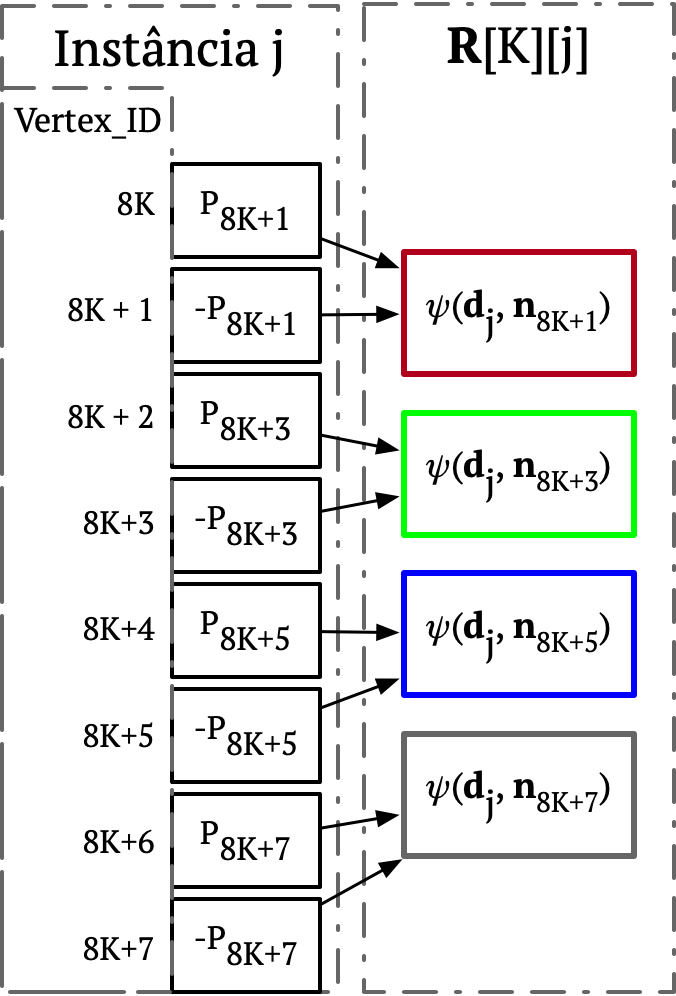
\includegraphics[width=.45\linewidth, angle=0]{figs/Esquema_Glifo/texellookup.png}
    \caption{Ilustração do acesso nas componentes RGBA em \textit{texel} na textura \textbf{R} no índice $K$ e $j$. O \textit{texel} é acessado pelas \textit{threads} que processam os vértices de índices 8K, 8K+1, ..., 8K+7 em uma instância $j$. Os blocos de contorno vermelho, azul, verde e cinza ilustram as componentes R,G,B e A do \textit{texel}, respectivamente.}
    \label{fig::texelfetch}
   %\hspace{1pt}
\end{figure}

\section{Processamento em GPU}
\label{sec::processamento_GPU}
\todo[inline]{Sugiro que detalhe um pouco mais a sua implementação de renderização usando os dois shaders. \textcolor{green}{OK!}}
\subsection{\textit{Vertex Shader}}

\subsubsection{Acesso dos dados de dODF min-max normalizados}
Os dados das dODFs min-max normalizadas são acessados no \textit{vertex shader}, quando cada glifo da $j$-ésima instância é processada. Os \textit{texels} com índice de coluna $K = \lfloor\frac{Vertex\_ID}{8} \rfloor$ são acessados para deslocar oito pontos. Usamos a função \textit{texelFetch} para acessar diretamente a textura de ODF utilizando coordenadas não-normalizadas $(j, \lfloor\frac{Vertex\_ID}{8} \rfloor)$. O valor utilizado para \textit{lookup} da componente  para deslocar o seu respectivo ponto na malha esférica no \textit{vertex shader} é acessível pela análise do resto da divisão por oito do Vertex\_ID, como ilustrado na Fig. \ref{fig::texelfetch}. Adicionalmente, utilizando a notação via colchetes, onde as componentes R, G, B e A são mapeados nos índices 0, 1, 2 e 3, respectivamente, o escalar de ODF pode ser mapeado por $\lfloor (Vertex\_ID \mod{8})/2 \rfloor$\footnote{A função em OpenGL para \textit{lookup} em função dos índices de instância e vértice é dada por texelFetch($\boldsymbol{\mathscr{R}}$,ivec2((gl\_VertexID)/8, gl\_InstanceID), 0)[(gl\_VertexID\%8)/2]}.


\subsubsection{Transformações geométricas}

Podemos sintetizar as transformações aplicadas a cada vértice $P_K$ em coordenadas homogêneas na $j$-ésima instância por uma multiplicação matricial por uma matriz $G_{Kj}$. Esta matriz pode ser sintetizada da seguinte forma:

\begin{equation}
    G_{Kj} = \mathbf{M_{vp}}\cdot M_D \cdot M_S \cdot M_{Kj}
\end{equation}
onde 
\begin{equation}
    M_{Kj} = \begin{bmatrix} 
   \mbox{\small $R( \mathbf{d}_j, \mathbf{n}_K)$} & 0 & 0 & 0 \\
    0 & \mbox{\small $R( \mathbf{d}_j, \mathbf{n}_K)$}  & 0 & 0 \\
    0 & 0 & \mbox{\small $R( \mathbf{d}_j, \mathbf{n}_K)$}  & 0 \\
    0 & 0 & 0 & 1 \\
\end{bmatrix},
\end{equation}
\begin{equation}
    M_{S} = \begin{bmatrix} 
    \frac{mS}{2} & 0             & 0            & 0 \\
    0            & \frac{mS}{2} & 0            & 0 \\
    0            & 0             & \frac{mS}{2} & 0 \\
    0            & 0             & 0            & 1 \\
\end{bmatrix},
\end{equation}
\begin{equation}
    M_{D} = \begin{bmatrix} 
    1 & 0 & 0 & dx \\
    0 & 1 & 0 & dy \\
    0 & 0 & 1 & dz \\
    0 & 0 & 0 & 1 \\
\end{bmatrix},
\end{equation}
e $\mathbf{M_{vp}}$ é a matriz \textit{view-projection}, que configura parâmetros de visão e projeção.

\subsection{\textit{Fragment Shader}}

No \textit{fragment shader} fazemos a definição de cor. Enviamos os valores absolutos das três componentes vértices da esfera unitária instanciada $(|P_x|, |P_y|, |P_z|)$ a partir do \textit{vertex shader} e atribuímos este valor a cor do fragmento, conforme Eq. \ref{eq::cor_glifo}.







